\section{Matching Circuits and Tuners}
\label{sec:tuners}

% Transmission line theory (reflection, max power transfer)
% [1] Pozar pp 56--57
% [2] Ebert p 29
% [3] Pozar pp 77--78
From transmission line theory, it is known that the voltage and current waves present on a transmission line is composed of an incident and a reflected wave. The voltage and current at any distance, $z$, from the load are \cite{pozar2011microwave}:
\begin{align}
    V(z) &= V^+e^{-j\beta z} + V^-e^{j\beta z}\\
    I(z) &= \frac{V^+}{Z_0} e^{-j\beta z} - \frac{V^-}{Z_0} e^{j\beta z}
\end{align}
where
\begin{where}
\item[$V(z)$] Voltage at distance $z$ [\si{V}]
\item[$I(z)$] Current at distance $z$ [\si{A}]
\item[$V^+$] Amplitude of the incident wave [\si{V}]
\item[$V^-$] Amplitude of the reflected wave [\si{V}]
\item[$Z_0$] Characteristic impedance of the transmission line [\si{\ohm}]
\item[$z$] Distance from load to the considered point [\si{m}]
\item[$\beta$] The wave number $=2\pi/\lambda$ [\si{rad\per m}]
\end{where}
The load impedance is the voltage-to-current ratio where $z=0$,
\begin{equation}
    Z_L = \frac{V(0)}{I(0)} = \frac{V^+ + V^-}{V^+ - V^-}Z_0
\end{equation}
Solving this for $V^-$ yields
\begin{equation}
    V^- = \frac{Z_L - Z_0}{Z_L + Z_0} V^+
\end{equation}
The ratio between the reflected and incident wave is known as the \emph{reflection coefficient}, denoted $\Gamma$,
\begin{equation}
    \label{eq:reflect}
    \Gamma = \frac{V^-}{V^+} = \frac{Z_L-Z_0}{Z_L+Z_0}
\end{equation}
Generally, the reflection coefficient along a transmission line can be written as \cite{ebert1998transmission}
\begin{equation}
    \Gamma(z) = \Gamma e^{j2\beta z}
\end{equation}
Note that $\Gamma$ without parameters indicates $\Gamma(0)$.

\begin{figure}[htbp]
    \centering
    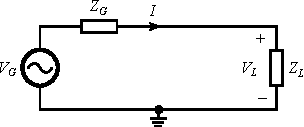
\includegraphics{img/analysis/generator_load}
    \caption{Equivalent circuit of a generator with given output impedance, $Z_G$, delivering power to a load of a given impedance, $Z_L$.}
    \label{fig:generator_load}
\end{figure}

To maximize the power transfered from a generator to a load, it is desired to have a reflection coefficient that is zero so that only forward waves are present on the transmission line. Figure~\ref{fig:generator_load} shows an equivalent circuit for this situation. The power in the load is found as \cite{pozar2011microwave}
\begin{equation}
    \label{eq:power1}
    P = \frac{1}{2} \real{V_LI^*} = \frac{1}{2} \real{\frac{|V_L|^2}{Z_L}}
    = \frac{1}{2} |V_L|^2 \real{\frac{1}{Z_L}}
\end{equation}
where
\begin{where}
\item[$P_L$] Power delivered to the load
\item[$V_L$] Voltage drop across the load
\item[$Z_L$] $R_L+jX_L$ is the load impedance
\item[$I$] Current through the load
\end{where}
Using basic circuit theory, Equation~\ref{eq:power1} can be expressed in terms of $V_G$ and $Z_G$, making it possible to derive the optimal $Z_G = R_G+jX_G$ for a fixed, complex load. Continuing from Equation~\ref{eq:power1},
\begin{equation}
    \begin{aligned}
        P &= \frac{1}{2} \left| V_G \frac{Z_L}{Z_L+Z_G} \right|^2 \real{\frac{1}{Z_L}} \\
        &= \frac{1}{2} |V_G|^2 \frac{|Z_L|^2}{|Z_L+Z_G|^2} \real{\frac{1}{Z_L}}\\
        &= \frac{|V_G|^2}{2} \frac{R_L^2+X_L^2}{(R_L+R_G)^2+(X_L+X_G)^2} \frac{R_L}{R_L^2 + X_L^2}\\
        &= \frac{|V_G|^2}{2} \frac{R_L}{(R_L+R_G)^2 + (X_L+X_G)^2}
    \end{aligned}
\end{equation}
The values of $R_G$ and $X_G$ that maximize the power delivered to the load, is found by 
\begin{enumerate}
\item Taking the partial derivative of $P$ with respect to $R_L$
\item Taking the partial derivative of $P$ with respect to $X_L$
\item Setting both of the above solutions equal to zero and solving for $R_G$ and $X_G$ (two equations with two unknowns)
    \begin{align}
        \dpd{P}{R_L} &= 0 \\
        \dpd{P}{X_L} &= 0
    \end{align}
\end{enumerate}
Doing so, yields the following solution,
\begin{equation}
    \begin{aligned}
        R_{G,\text{max}} &= R_L \\
        X_{G,\text{max}} &= -X_L
    \end{aligned}
\end{equation}
or $Z_{G,\text{max}} = Z^*_L$; the maximum power is transfered to the load when the generator impedance is the complex conjugate of the load impedance. In this situation the generator is said to be \emph{matched} to the load. Generally, the generator and the load would be connected through a transmission line with the characteristic impedance $Z_0$, so the maximum power transfer from generator to load will occur when both generator and load are matched to $Z_0$. 

% Mismatch loss, S11. |S11| = -6 dB  -->  SWR = 3
\begin{figure}[htbp]
    \centering
    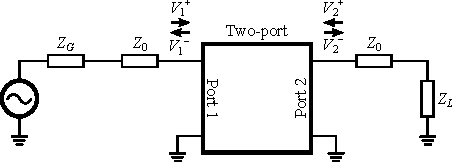
\includegraphics{img/analysis/s_parameter_twoport}
    \caption{S-parameters of a two-port system.}
    \label{fig:twoport}
\end{figure}

The reflection coefficient, $\Gamma$, can more generally be described as an \emph{S-parameter}. The S-parameters describe the ratio between the reflected and incident wave at a given port in a system. Consider a two-port as shown in Figure~\ref{fig:twoport}. Its four S-parameters are defined as follows:
\begin{align*}
    &S_{11} = \frac{V_1^-}{V_1^+} \Bigg|_{V_2^+=0} = \Gamma_1
    &&S_{12} = \frac{V_1^-}{V_2^+} \Bigg|_{V_1^+=0} \\
    &S_{21} = \frac{V_2^-}{V_1^+} \Bigg|_{V_2^+=0}
    &&S_{22} = \frac{V_2^-}{V_2^+} \Bigg|_{V_1^+=0} = \Gamma_2
\end{align*}
It is seen that $S_{11}$ and $S_{22}$ indicate the reflection due to the incident wave on the same port, when no contribution is made from the opposite port, i.e., these are the reflection coefficients of port 1 and 2, respectively. The parameter $S_{21}$ indicates how much of the incident wave on port 1 is coming out of port 2 when no wave is incident on port 2, i.e., this indicates the \emph{transmission coefficient} from port 1 to port 2. Likewise, $S_{12}$ is the transmission coefficient from port 2 to port 1.

The S-parameters are easily measured using a Vector Network Analyzer (VNA). The advantage of measuring S-parameters over, e.g., Y-parameters is that all ports are matched during the measurement instead of some being shorted, making odd behavior (like oscillations) less likely \cite{Bowick2007}.

% Smith chart visualization
\begin{figure}[htbp]
    \centering
    \begin{tikzpicture}
        \begin{smithchart}[mark repeat=3]
            \addplot coordinates {
                (0.5,0.2) 
                (0.5,0.3)
                (0.5,0.4)
                (0.5,0.5)
            };
            \path[draw=black, very thick] (0pt,0pt) circle (14.3mm);
        \end{smithchart}
    \end{tikzpicture}
    \caption{Smithchart. The circle illustrates the limit for which all points within the circle have a reflection coefficient below $\Gamma=0.5$ (or \SI{-6}{dB}). Two points -- $0.5+j0.2$ and $0.5+j0.5$ -- are shown.}
    \label{fig:smithchart}
\end{figure}
An important tool when doing matching, and designing antennas, to a certain $Z_0$ is the smith chart. The smith chart is used for plotting complex, normalized impedances and makes it easy to visually analyze the performance of a matched circuit. A smith chart is shown in Figure~\ref{fig:smithchart}.

The smith chart maps the entire right complex half-plane into a circle, having $0+j0$ all the way to the left and $\infty+j0$ all the way to the right. The y-axis (crossing $x=0$) makes up the circumference of the circle. An impedance is plotted by first finding the resistive (real) part of the impedance on the horizontal line and then following the circular grid-lines up or down for positive or negative reactances, respectively. 
The smith chart shown in Figure~\ref{fig:smithchart} is a normalized smith chart. When matching to $Z_0$, any impedance, $Z$, plotted in the smith chart, must be normalized by $Z_0$:
\begin{equation}
    Z_n = \frac{Z}{Z_0}
\end{equation}
This means that $Z_0$ will always appear at $1+j0$ -- in the center of the smith chart -- and the goal of the matching is to get the impedance of the antenna (or other circuitry) as close to the center as possible for the desired frequency range.

The impedance bandwidth of an antenna is often given as the bandwidth for which the reflection coefficient, $\Gamma$, is below 0.5 (or \SI{-6}{dB} -- when denoting the reflection coefficient in decibels, it is commonly called \emph{return loss}). It may therefore be advantageous to plot this requirement. In the smith chart, this is plotted as a circle around the center and any point within the circle, is within the bandwidth of the circuit. The \SI{-6}{dB} circle is also shown in Figure~\ref{fig:smithchart}. This type of circle is also known as a SWR (Standing Wave Ratio) circle. The connection between the SWR and the reflection coefficient is \cite{pozar2011microwave}
\begin{equation}
    \text{SWR} = \frac{1 + |\Gamma|}{1 - |\Gamma|}
\end{equation}
At $\Gamma = \SI{-6}{dB}$, the SWR is 3.

% Matching circuitry, L-network, smith chart ``ups and downs'', analytical formulas.
\subsection{The L Network}
\begin{figure}[htbp]
    \begin{subfigure}{0.49\linewidth}
        \centering
        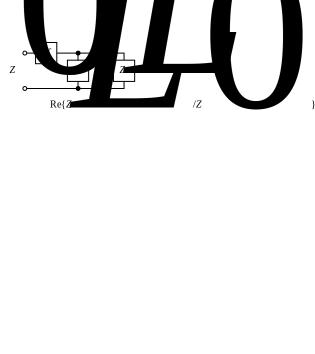
\includegraphics{img/analysis/l_network_a}
        \caption{Real part of normalized load impedance greater than one.}
        \label{fig:l_network_a}
    \end{subfigure}
    \hfill
    \begin{subfigure}{0.49\linewidth}
        \centering
        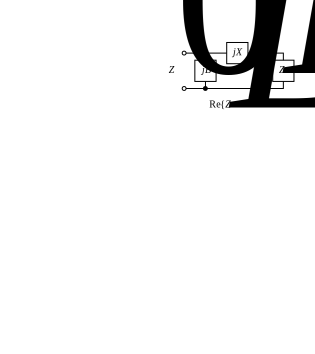
\includegraphics{img/analysis/l_network_b}
        \caption{Real part of normalized load impedance less than one.}
        \label{fig:l_network_b}
    \end{subfigure}
    \caption{L-network. The series/shunt configuration depends on the value of the load impedance.}
    \label{fig:l_network}
\end{figure}
In case the antenna is not designed to resonate exactly at the desired frequency or to the exact impedance bandwidth required, a tuning network can be placed immediately before the antenna. 

The simplest matching network is the L-network which is made from two components -- one in series an one in shunt -- as shown in Figure~\ref{fig:l_network}. The values of $X$ and $B$ correspond to the reactance of the chosen component at the frequency of interest. The values of $X$ and $B$ (and their corresponding component values) can be derived through circuit theory, as done by \cite{pozar2011microwave}. The results are shown in Table~\ref{tab:match_XB}.

\def\TabSpace{\rule{0pt}{4ex} \rule[-2.5ex]{0pt}{0pt}}
\begin{table}[htbp]
    \centering
    \begin{tabular}{|c|c|c|c|}
        \hline
        \textbf{Variable} & \textbf{Description} & \textbf{Figure~\ref{fig:l_network_a}} & \textbf{Figure~\ref{fig:l_network_b}} \\
        \hline
        \TabSpace $Z_n$ & Normalized load $=R_n+jX_n$ & \multicolumn{2}{c|}{$Z_L/Z_0$}\\ \hline
        \TabSpace $b$ & Normalized shunt susceptance $=BZ_0$ & $\dfrac{X_n \pm \sqrt{R_n}\sqrt{R_n^2 + X_n^2 - R_n}}{R_n^2+X_n^2}$ & $\pm\sqrt{(1-R_n)/R_n}$\\ \hline
        \TabSpace $x$ & Normalized series reactance = $X/Z_0$ & $\dfrac{1}{b} + \dfrac{X_n}{R_n} - \dfrac{1}{bR_n}$ & $- X_n \pm \sqrt{R_n(1-R_n)}$\\ \hline
        \TabSpace $C_p$ & Shunt capacitance in farad (for $b>0$) & \multicolumn{2}{c|}{ $\dfrac{b}{2\pi f Z_0}$ } \\ \hline
        \TabSpace $L_p$ & Shunt inductance in henry (for $b<0$) & \multicolumn{2}{c|}{ $\dfrac{-Z_0}{2\pi f b}$ } \\ \hline
        \TabSpace $C_s$ & Series capacitance in farad (for $x<0$) & \multicolumn{2}{c|}{ $\dfrac{-1}{2\pi f x Z_0}$} \\ \hline
        \TabSpace $L_s$ & Series inductance in henry (for $x>0$) & \multicolumn{2}{c|}{ $\dfrac{xZ_0}{2\pi f}$} \\ \hline
    \end{tabular}
    \caption{Formulas for computing the values of matching components for the two matching networks shown in Figure~\ref{fig:l_network}. These L-networks match a load (or antenna) impedance, $Z_L$ ohm to a transmission line, $Z_0$ ohm at the frequency $f$ hertz. There are two solutions: One for choosing $\pm=+$ and one for choosing $\pm=-$ \cite{pozar2011microwave}.}
    \label{tab:match_XB}
\end{table}

\subsection{Q Factor}
The Q factor describes the ratio between the reactive and the resistive part of a component,
\begin{equation}
    \label{fig:compq}
    Q = \frac{X}{R}
\end{equation}
where $X$ is the reactance of the component and $R$ is the resistive part of the component. Ideal capacitors and inductors are purely reactive and therefore, no power is lost in them (the average power $P = \real{VI*} = |V|^2 / \real{Z}$ only depends on the real part of $Z$ \cite{irwin2011engineering}). However, practical components also has a small resistive part called the equivalent series resistance (ESR) which causes power to be transfered to the component, increasing the power loss. From Equation~\ref{fig:compq}, it is therefore seen that a \emph{large} Q factor is desired for capacitors and inductors. The Q factor of an antenna should, however, not necessarily be large as it is desired to lose power due to radiation, but a low Q factor is not necessarily a good thing either, as the power loss may be caused by resistive loss in the antenna and not radiation.

% Tuners: Series capacitor, shunt capacitor, variable inductor?
\subsection{Tuners}
From the description above it is seen that the resonance frequency of an antenna can be altered by changing the matching network. By replacing a fixed capacitor with a variable capacitor it is possible to cover a broader total bandwidth by tuning the resonance frequency. As the achievable bandwidth is generally proportional to the size of the antenna \fixme{Reference to Henrik's section?}, it will be possible to cover a large bandwidth using a physically smaller antenna by having a variable matching network. This is desirable for mobile phones where the physical size of the antenna is limited and multiple bands must be covered \cite{gu2014rf}.

\subsubsection{Variable Capacitors}
Three basic types of variable capacitors will now be described briefly. 

Barium strontium titanate (BST) varactors are voltage controlled components where the bias voltage determines the amount of capacitance provided by the component. The Q factor is dependent on the tuning range, $\eta$. For a tuning range of $\eta = 2--4$ at around \SI{3}{GHz}, the Q factor is around 30--65 \cite{gu2014rf}. 

A downside of the BST varactor is that it is quite nonlinear, having a typical third order intercept point ($\text{IIP}_3$) of around 32--\SI{40}{dBm} \cite{gu2014rf}. Also, an external power supply is necessary to bias the varactor.

Another type of variable capacitor is a SOI/SOS digitally tunable capacitor (SOI $=$ silicon on isolator switches, SOS $=$ silicon on sapphire switches). These consist of metal-isolator-metal (MIM) capacitors which are digitally switched using CMOS SOI or SOS switches as shown in Figure~\ref{fig:sossoiswitch}. 

The Q factor around \SI{2}{GHz} of SOS/SOI digitally tunable capacitors (DTC) is typically 40--50 at minimum capacitance and $\geq$ 15 at maximum capacitance \cite{gu2014rf}. This is generally worse than the BTS varactors. The linearity, however, is generally better than for the BTS varactors with an $\text{IIP}_3$ of around \SI{44}{dBm} \cite{gu2014rf}.

\begin{figure}[htbp]
    \centering
    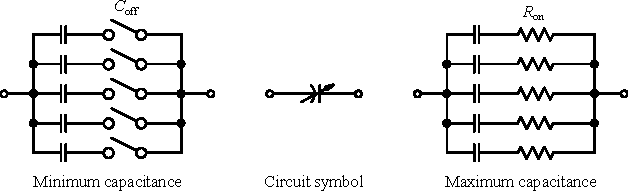
\includegraphics{img/analysis/sossoi_dtc}
    \caption{Circuit showing the operation of a SOS/SOI digitally tunable capacitor. To the left, the minimum capacitance situation is shown, where only parasitic capacitance from the switches is present. To the right, the maximum capacitance situation is shown where the on-resistance of the switches degrades the Q factor.}
    \label{fig:sossoiswitch}
\end{figure}

A big advantage of the SOI/SOS DTCs is that their control voltage is less than \SI{5}{V} and that they are quite low cost \cite{gu2014rf}.

The last type of capacitor described is a MEMS tunable capacitor, which is the type used for this project. The MEMS tunable capacitor cell is shown in Figure~\ref{fig:memscap}.

A MEMS tunable capacitor consists of several of the cells shown in Figure~\ref{fig:memscap}. By applying a voltage on one or more of the cells, the top plate is pulled toward the bottom electrode, increasing the overall capacitance. 

The Q factor of a MEMS tunable capacitor is much higher than that of the BTS varactor and the SOI/SOS DTS -- typically higher than 200 at minimum capacitance and above 100 at maximum capacitance, at \SI{2}{GHz} \cite{gu2014rf}. The linearity is also better, having an achievable $\text{IIP}_3$ of greater than \SI{68}{dBm} at \SI{2.5}{GHz}. 

\begin{figure}[htbp]
    \centering
    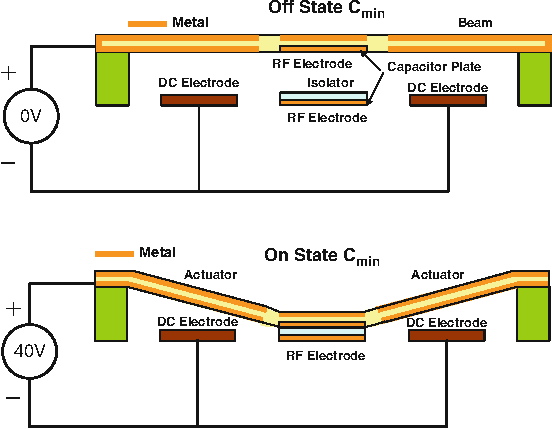
\includegraphics{img/analysis/memscap}
    \caption{MEMS tunable capacitor cell in the on and off state \cite{gu2014rf}.}
    \label{fig:memscap}
\end{figure}

\subsubsection{Tuner Modeling}
% [Gu Sec 2.1 and 2.2], [Bowick RF]: S-parameters --> component values

\def\TabSpace{\rule{0pt}{4.5ex} \rule[-3ex]{0pt}{0pt}}
\def\refmistake{$^{\dagger}$}
\begin{table}
    \centering
    \begin{tabular}{|l|c|c|}
        \hline
        & Series capacitor ($\pi$) & Shunt capacitor (T) \\
        \hline
        \rule{0pt}{12ex} \rule[-12ex]{0pt}{0pt}Circuit & \raisebox{-.5\height}{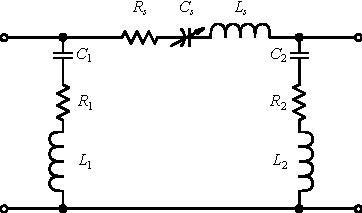
\includegraphics{img/analysis/pi_network}} & \raisebox{-.5\height}{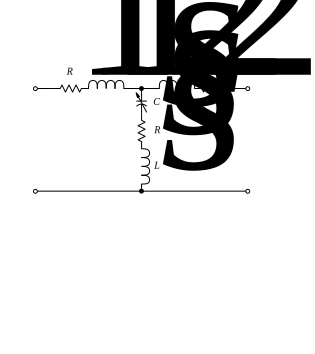
\includegraphics{img/analysis/T_network}} \\
        \hline
        \TabSpace$\omega_L$  & \multicolumn{2}{c|}{$2\pi f_{\text{low}}$} \\
        \TabSpace$\omega_H$  & \multicolumn{2}{c|}{$2\pi f_{\text{high}}$} \\
        \hline
        \TabSpace$X_1(\omega)$ 
        & $Z_0\imag{\dfrac{1+S_{11}+S_{22}+(S_{11}S_{22}-S_{21}^2)}{1+S_{22}-S_{11}-2S_{21}-(S_{11}S_{22}-S_{21}^2)}}$ 
        & $Z_0 \imag{\dfrac{1+S_{11}-S_{22}-2S_{21}-(S_{11}S_{22}-S_{21}^2)}{1-S_{11}-S_{22}+(S_{11}S_{22}-S_{21}^2)}}$\\
        \TabSpace$X_S(\omega)$ 
        & $Z_0 \imag{\dfrac{1+S_{11}+S_{22}+S_{11}S_{22}-S_{21}^2}{2S_{21}}}$ \refmistake
        & $Z_0 \imag{\dfrac{2S_{21}}{1-S_{11}-S_{22}+S_{11}S_{22}-S_{21}^2}}$\\
        \TabSpace$X_2(\omega)$ 
        & $Z_0 \imag{\dfrac{1 + S_{11} + S_{22} + (S_{11}S_{22}-S_{21}^2)}{1 + S_{11} - S_{22} - 2S_{21} - (S_{11}S_{22} - S_{21}^2)}}$ 
        & $Z_0 \imag{\dfrac{1-S_{11}+S_{22}-2S_{21}-(S_{11}S_{22}-S_{21}^2)}{1-S_{11}-S_{22}+(S_{11}S_{22}-S_{21}^2)}}$\\
        \hline
        \TabSpace$L_k$ 
        & $\dfrac{\omega_LX_k(\omega_L) - \omega_HX_k(\omega_H)}{\omega_L^2-\omega_H^2}$ \refmistake
        &  \\
        \TabSpace$C_k$ 
        & $\dfrac{\omega_L^2-\omega_H^2}{\omega_L\omega_H} \dfrac{1}{\omega_HX_k(\omega_L) - \omega_LX_k(\omega_H)}$
        &  \\
        \hline
        \TabSpace$R_1$ 
        & $Z_0 \real{\dfrac{1+S_{11}+S_{22}+(S_{11}S_{22}-S_{21}^2)}{1+S_{22}-S_{11}-2S_{21}-(S_{11}S_{22}-S_{21}^2)}}$ 
        & $Z_0 \real{\dfrac{1+S_{11}-S_{22}-2S_{21}-(S_{11}S_{22}-S_{21}^2}{1-S_{11}-S_{22}+(S_{11}S_{22}-S_{21}^2)}}$\\
        \TabSpace$L_1$ 
        & $L_k\Big|_{k=1}$ 
        & $\dfrac{Z_0}{\omega} \imag{\dfrac{1+S_{11}-S_{22}-2S_{21}-(S_{11}S_{22}-S_{21}^2)}{1-S_{11}-S_{22}+(S_{11}S_{22}-S_{21}^2)}}$\\
        \TabSpace$C_1$ 
        & $C_k\Big|_{k=1}$ 
        & \\
        \hline
        \TabSpace$R_s$ 
        & $Z_0 \real{\dfrac{1+S_{11}+S_{22}+S_{11}S_{22}-S_{21}^2}{2S_{21}}}$ 
        & $Z_0 \real{\dfrac{2S_{21}}{1-S_{11}-S_{22}+S_{11}S_{22}-S_{21}^2}}$\\
        \TabSpace$L_s$ 
        & $L_k\Big|_{k=s}$ 
        & $\dfrac{\omega_LX_s(\omega_L) - \omega_HX_s(\omega_H)}{\omega_L^2 - \omega_H^2}$\\
        \TabSpace$C_s$ 
        & $C_k\Big|_{k=s}$ 
        & $\dfrac{\omega_L^2 - \omega_H^2}{\omega_L\omega_H} \dfrac{1}{\omega_HX_s(\omega_L) - \omega_LX_s(\omega_H)}$\\
        \hline
        \TabSpace$R_2$ 
        & $Z_0 \real{\dfrac{1+S_{11}+S_{22}+(S_{11}S_{22}-S_{21}^2)}{1+S_{11}-S_{22}-2S_{21}-(S_{11}S_{22}-S_{21}^2)}}$ \refmistake
        & $Z_0 \real{\dfrac{1-S_{11}+S_{22}-2S_{21}-(S_{11}S_{22}-S_{21}^2)}{1-S_{11}-S_{22}+(S_{11}S_{22}-S_{21}^2)}}$\\
        \TabSpace$L_2$ 
        & $L_k\Big|_{k=2}$ 
        & $\dfrac{Z_0}{\omega} \imag{\dfrac{1-S_{11}+S_{22}-2S_{21}-(S_{11}S_{22}-S_{21}^2)}{1-S_{11}-S_{22}+(S_{11}S_{22}-S_{21}^2)}}$\\
        \TabSpace$C_2$ 
        & $C_k\Big|_{k=2}$ 
        & \\
        \hline
    \end{tabular}
    \caption{Formulas for computing the equivalent circuit components from S-parameters measured at two frequencies, $f_{\text{low}}$ and $f_{\text{high}}$ \cite{gu2014rf}. Here $\omega$ with no index indicated the angular frequency of calculation. The resistance values may change depending on the frequency of the S-parameter measurement. \refmistake Mistakes in reference \fixme{Delete this?}.}
    \label{tab:sparam_to_circuit}
\end{table}

% Insertion loss, S21 for networks, equivalent series resistance, component Q.
